\documentclass[aspectratio=169]{beamer}
\usepackage[utf8]{inputenc}
\usepackage{graphicx}
\graphicspath{{images/}}
\usepackage{booktabs}
\usepackage{tcolorbox}
\usepackage{tikz}
\usepackage{amsmath}
\usepackage{colortbl}
\usepackage{amssymb}
\usetikzlibrary{shapes.geometric, arrows.meta, positioning, calc, shadows}

\usepackage{mathptmx}
\usefonttheme{serif}

% Colors
\definecolor{main}{RGB}{0,150,136}    % Primary Teal
\definecolor{boldblue}{RGB}{0,51,153} % Bold Royal Blue for Title
\definecolor{footertext}{RGB}{100,100,100} % Professional Gray for footer

% Unified theme colors
\definecolor{tda}{RGB}{0,150,136} 

% Box style - Set backgrounds to WHITE
\tcbset{
    mybox/.style={
        colback=white,
        colframe=main,
        arc=5pt,
        boxrule=1pt,
        fonttitle=\bfseries\small,
        left=2pt, right=2pt, top=2pt, bottom=2pt
    },
    tdabox/.style={
        colback=white,
        colframe=main,
        arc=5pt,
        boxrule=1pt,
        fonttitle=\bfseries\small
    }
}

% Navigation
\setbeamertemplate{navigation symbols}{}
\setbeamertemplate{footline}{
    \begin{beamercolorbox}[wd=\paperwidth,ht=2ex,dp=1.2ex,leftskip=0.5cm,rightskip=0.5cm]{white}
        \fontsize{5pt}{6pt}\selectfont
        \color{boldblue}\textbf{\raisebox{-0.5pt}{Arjeet Singh --- IIIT Manipur}}
        \hfill \color{main}\raisebox{-0.5pt}{\insertframenumber/6}
    \end{beamercolorbox}
}

% Bold Blue Title for impact
\title{\color{boldblue}\textbf{Emotion Detection from Textual Data}}
\subtitle{\color{boldblue}with Ambiguity Detection}
\author{\textbf{Arjeet Singh (230101078)}}
\institute{
    Under the supervision of: \\
    \textbf{Dr. Rajkumari Bidyalakshmi Devi} \\
    \vspace{0.3cm}
    Department of CSE \\ IIIT Manipur
}
\date{April 2026}

\begin{document}

%---------------- Title Slide ----------------%
\begin{frame}[label=title]
\titlepage
\end{frame}

%---------------- Slide 1: Introduction, Objective \& Contribution ----------------%
\begin{frame}[label=slide1]{Slide 1: Introduction, Objective \& Contribution}
\begin{tcolorbox}[mybox,title=Introduction]
\scriptsize
\begin{itemize}
    \item Formal textual corpora are primary hubs for structured emotional expression.
    \item Textual content is often formal, yet can be inherently ambiguous in certain contexts.
    \item Standard NLP models often provide unreliable results due to forced classification on unclear text.
\end{itemize}
\end{tcolorbox}

\vspace{0.2cm}

\begin{columns}[T]
\begin{column}{0.48\textwidth}
\begin{tcolorbox}[mybox,title=Objectives,height=3.8cm]
\scriptsize
\begin{itemize}
    \item Map GoEmotions dataset (28 classes) to Positive, Negative, and Neutral labels.
    \item Develop a robust classification pipeline using ensemble XGBoost models.
    \item Implement an explicit ambiguity detection mechanism to identify uncertain inputs.
\end{itemize}
\end{tcolorbox}
\end{column}

\begin{column}{0.48\textwidth}
\begin{tcolorbox}[tdabox,title=Key Contribution,height=3.8cm]
\scriptsize
\begin{itemize}
    \item Integrated \textbf{Topological Data Analysis (TDA)} to analyze the geometric distribution of dense embeddings.
    \item Defined \textbf{H1 Loop count} as a structural metric for identifying boundary complexity.
    \item Enabled principled abstention by flagging \textbf{Ambiguous} cases based on data geometry.
\end{itemize}
\end{tcolorbox}
\end{column}
\end{columns}
\end{frame}

%---------------- Slide 2: Related Work \& Motivation ----------------%
\begin{frame}[label=slide2]{Slide 2: Related Work \& Motivation}
\vspace*{-0.4cm}
\begin{columns}[T]
\begin{column}{0.48\textwidth}
\begin{tcolorbox}[mybox,title=What Others Have Done,height=3.6cm]
\scriptsize
\begin{itemize}
    \item \textbf{BERT (baseline)}: $\to$ \textbf{~0.46} Macro-F1
    \item \textbf{SBERT}: $\to$ \textbf{~82\%} accuracy
    \item \textbf{Recent Transformers}: $\to$ \textbf{~86--87\%} accuracy
    \item \textbf{BiLSTM (2021)}: $\to$ Macro-F1 \textbf{$\sim$ 0.45}
    \item \textbf{LLM-based (2023)}: $\to$ Accuracy \textbf{$\sim$ 85\%}
\end{itemize}
\end{tcolorbox}

\vspace*{-0.1cm}

\begin{tcolorbox}[mybox,title=Why Your Project is Needed,height=3.6cm]
\scriptsize
\begin{itemize}
    \item \textbf{Authenticity}: Real-world formal text can be genuinely ambiguous --- forcing a label is misleading.
    \item \textbf{Trust}: Mental health monitoring needs to know when a prediction shouldn't be trusted.
    \item \textbf{Gap}: No existing GoEmotions system has an explicit \textbf{Ambiguous} output.
\end{itemize}
\end{tcolorbox}
\end{column}

\begin{column}{0.48\textwidth}
\begin{tcolorbox}[mybox,title=Problems with Existing Work,height=3.6cm]
\scriptsize
\begin{itemize}
    \item \textbf{No Abstention}: No system can say ``I don't know''.
    \item \textbf{Contextual}: Fail on nuanced expressions (e.g., ``I am fine'').
    \item \textbf{Imbalance}: Poor on minority classes.
    \item \textbf{Bias}: Confidence methods rely on biased models.
\end{itemize}
\end{tcolorbox}

\vspace*{-0.1cm}

\begin{tcolorbox}[tdabox,title=How Your Project Solves It,height=3.6cm]
\scriptsize
\begin{itemize}
    \item \textbf{New Output}: Adds \textbf{Ambiguous} class to avoid forced errors.
    \item \textbf{Structural TDA}: Uses persistent homology to capture complexity, independent of model bias.
    \item \textbf{Hybrid Signal}: Combines topology + confidence gap.
\end{itemize}
\end{tcolorbox}
\end{column}
\end{columns}
\end{frame}

%---------------- Slide 3: Proposed System / Architecture ----------------%
\begin{frame}[label=slide3]{Slide 3: Proposed System / Architecture}
\vspace*{-0.3cm}
\begin{tcolorbox}[mybox,title=Tools Used (Software \& Environment),height=2.3cm,width=\textwidth]
\scriptsize
\setbeamertemplate{itemize item}{\color{boldblue}$\blacktriangleright$}
\begin{columns}[T]
\begin{column}{0.49\textwidth}
\begin{itemize}
    \item \textbf{Python 3.10+}: Core Development
    \item \textbf{SentenceTransformers}: Embeddings
    \item \textbf{Giotto-TDA}: Homology computation
\end{itemize}
\end{column}
\begin{column}{0.49\textwidth}
\begin{itemize}
    \item \textbf{XGBoost}: Multi-class classification
    \item \textbf{Scikit-Learn}: TF-IDF \& pipelines
    \item \textbf{Pandas/NumPy}: Data processing
\end{itemize}
\end{column}
\end{columns}
\end{tcolorbox}

\vspace*{-0.1cm}

\begin{columns}[T]
\begin{column}{0.28\textwidth}
\centering
\vspace*{-0.1cm}
\hspace*{-0.6cm}
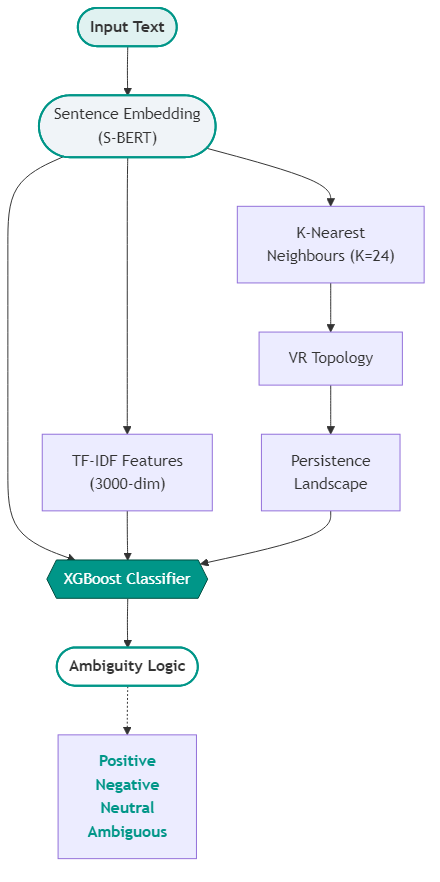
\includegraphics[width=1.1\linewidth,height=4.8cm,keepaspectratio]{system_architecture.png}
\end{column}

\begin{column}{0.29\textwidth}
\vspace{-0.1cm}
\begin{tcolorbox}[tdabox,title=Decision Logic,height=4.9cm]
\fontsize{7.5pt}{12pt}\selectfont
\begin{itemize}
    \item If loop $\ge$ 14 $\to$ \textbf{Ambiguous}
    \item If loop $\ge$ 10 \& gap $<$ 0.30 $\to$ \textbf{Ambiguous}
    \item If gap $<$ 0.10 $\to$ \textbf{Ambiguous}
    \item Else $\to$ \textbf{Predicted class}
\end{itemize}
\end{tcolorbox}
\end{column}

\begin{column}{0.38\textwidth}
\vspace{-0.1cm}
\begin{tcolorbox}[mybox,title=Steps Involved (Workflow),height=4.9cm]
\fontsize{7pt}{10.5pt}\selectfont
\begin{itemize}
    \item \textbf{1. Mapping}: GoEmotions $\to$ Pos/Neg/Neu.
    \item \textbf{2. Embed}: Text $\to$ 768-dim via S-BERT.
    \item \textbf{3. Context}: Identify 24 neighbours.
    \item \textbf{4. TDA}: VR complex + $H_1$ ($\epsilon$ birth--death) + landscape.
    \item \textbf{5. Fusion}: Embeds + TF-IDF + TDA.
    \item \textbf{6. Ensemble}: Classify via XGBoost.
    \item \textbf{7. Logic}: Flag \textbf{Ambiguous} if rules met.
\end{itemize}
\end{tcolorbox}
\end{column}
\end{columns}
\end{frame}

%---------------- Slide 4: Results & Analysis ----------------%
\begin{frame}[t,label=slide4]{Slide 4: Result \& Analysis}
\vspace{0.05cm}
\begin{columns}[T]
\begin{column}{0.38\textwidth}
\vspace{0.05cm}
\scriptsize
\textbf{Experimental Setup:}
\begin{itemize}
    \item \textbf{Training}: 43,410 samples
    \item \textbf{Testing}: 5,427 samples
    \item \textbf{Accuracy}: 59\%
\end{itemize}

\vspace{0.1cm}
\textbf{Classification Performance:}
\renewcommand{\arraystretch}{1.0}
\centering
\begin{tabular}{lcccc}
\toprule
\textbf{Class} & \textbf{Prec.} & \textbf{Rec.} & \textbf{F1} \\
\midrule
Positive & 0.54 & 0.83 & 0.65 \\
Negative & 0.28 & 0.65 & 0.39 \\
Neutral & 0.86 & 0.49 & 0.63 \\
\bottomrule
\end{tabular}
\end{column}

\begin{column}{0.60\textwidth}
\vspace{0.2cm}
\scriptsize
\centering
\textbf{Comparative Performance:}
\renewcommand{\arraystretch}{1.2}
\setlength{\tabcolsep}{4pt}
\begin{tabular}{|l|c|c|}
\hline
\textbf{Model} & \textbf{Accuracy} & \textbf{Ambiguity Det.} \\ \hline
BERT-based Models & $\sim$85\% & No \\ \hline
Sentence-BERT & $\sim$82\% & No \\ \hline
Transformer Variants & $\sim$86--87\% & No \\ \hline
\textbf{Proposed Model} & \textbf{59\%} & \textbf{Yes (Explicit)} \\ \hline
\end{tabular}
\end{column}
\end{columns}

\vfill

\begin{tcolorbox}[tdabox,title=Findings \& Qualitative Examples]
\vspace{-0.1cm}
\begin{columns}[T]
\begin{column}{0.48\textwidth}
\scriptsize
\begin{itemize}
    \item TDA identifies ambiguous inputs via geometric structure.
    \item Flags uncertain inputs as \textbf{Ambiguous} (Loops $\ge$ 14 or Gap $<$ 0.10).
    \item Complements ML confidence signals to avoid wrong predictions.
\end{itemize}
\end{column}
\begin{column}{0.48\textwidth}
\scriptsize
\centering
\renewcommand{\arraystretch}{1.1}
\setlength{\tabcolsep}{3pt}
\begin{tabular}{lccc}
\toprule
\textbf{Input} & \textbf{Loops} & \textbf{Gap} & \textbf{Result} \\
\midrule
``I am very happy'' & 4 & 0.40 & POSITIVE \\
``I dont know how I feel'' & 15 & 0.15 & AMBIGUOUS \\
``I will kill you'' & 4 & 0.06 & AMBIGUOUS \\
\bottomrule
\end{tabular}
\end{column}
\end{columns}
\end{tcolorbox}
\end{frame}

%---------------- Slide 5: Conclusion ----------------%
\begin{frame}[t,label=slide5]{Slide 5: Conclusion}
\vspace*{-0.2cm}
\begin{tcolorbox}[mybox,title=Summary of Achievements]
\scriptsize
\begin{itemize}
    \item Developed a working emotion detection pipeline achieving 59\% accuracy.
    \item Implemented a novel topological ambiguity detection layer using H1 loop counts.
    \item Identified complex boundary cases like ``i dont know how i feel'' (Loops: 15).
    \item Demonstrated that TDA identifies ambiguous text where standard models struggle.
\end{itemize}
\end{tcolorbox}

\vspace*{-0.3cm}

\begin{columns}[T]
\begin{column}{0.48\textwidth}
\begin{tcolorbox}[mybox,title=Limitations,height=4.4cm]
\scriptsize
\begin{itemize}
    \item \textbf{Ambiguity}: Sarcasm not reliably detected  
    \item \textbf{Latency}: 2--4s per query  
    \item \textbf{Language}: English-only bias  
    \item \textbf{Slang}: Poor handling of internet slang
    \item \textbf{Domain}: Features tied to GoEmotions geometry
    \item \textbf{Memory}: No tracking of user interaction history
\end{itemize}
\end{tcolorbox}
\end{column}

\begin{column}{0.48\textwidth}
\begin{tcolorbox}[tdabox,title=Future Work,height=4.4cm]
\scriptsize
\begin{itemize}
    \item \textbf{Labeled Data}: Human-annotated ambiguity dataset  
    \item \textbf{28-Class}: Full GoEmotions expansion  
    \item \textbf{Sarcasm}: Dedicated irony detection  
    \item \textbf{Speed}: Precomputed topological features  
    \item \textbf{Multilingual}: Cross-language embeddings
\end{itemize}
\end{tcolorbox}
\end{column}
\end{columns}
\end{frame}

\end{document}
